\documentclass[10pt,a4paper]{article}
\usepackage[T1]{fontenc}
\usepackage{lmodern}
\usepackage[margin=23mm]{geometry}
\usepackage{amsmath,amssymb,booktabs,microtype,tikz}
\usepackage[hidelinks]{hyperref}
\usetikzlibrary{arrows.meta,positioning}
\pdfinfoomitdate=1
\pdftrailerid{}
\pdfsuppressptexinfo=15
\setlength{\parindent}{0pt}
\setlength{\parskip}{5pt}
\title{From an extended hydrogen atom to an H-alpha spectrum}
\author{\texttt{exojax-escape}: model definition and numerical verification}
\date{Definition revision 1; 22 November 2026}
\begin{document}
\maketitle

\section{What is connected}
The extended atom used in the local Cloudy comparisons now also supplies the
observer spectrum. It resolves $1s,2s,2p,3s,3p,3d$ and includes statistical
shells $n=4,\ldots,15$: eighteen bound populations plus ionization. Increasing
the cutoff to 20 is a numerical control. There is no fitted correction to the
excited populations. In particular, $n_3=n_{3s}+n_{3p}+n_{3d}$ excludes every
higher shell even though cascades from those shells change its value.

\begin{center}
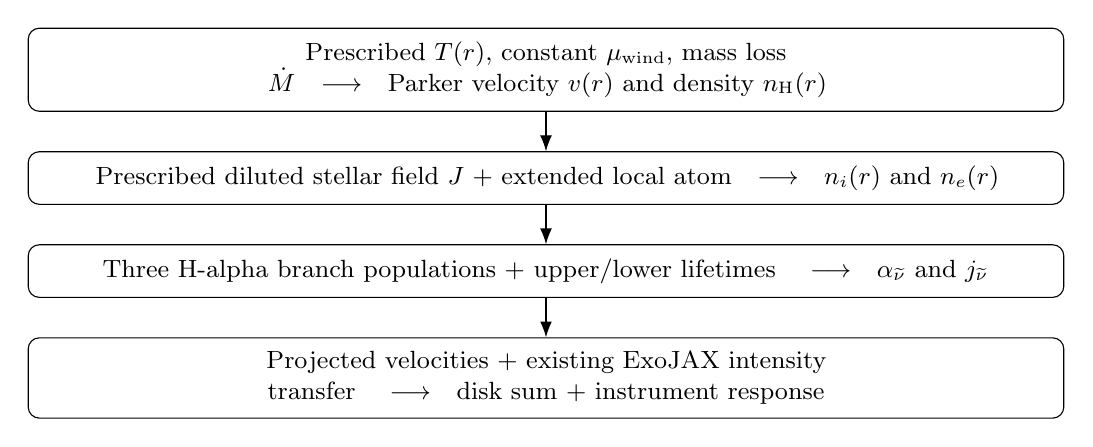
\begin{tikzpicture}[node distance=5mm,
  box/.style={draw,rounded corners,align=center,text width=12.8cm,
              inner sep=5pt,font=\small},arr/.style={-{Latex[length=2mm]}}]
\node[box] (wind) {Prescribed $T(r)$, constant $\mu_{\rm wind}$, mass loss
  $\dot M$\quad$\longrightarrow$\quad Parker velocity $v(r)$ and density $n_{\rm H}(r)$};
\node[box,below=of wind] (atom) {Prescribed diluted stellar field $J$
  + extended local atom\quad$\longrightarrow$\quad$n_i(r)$ and $n_e(r)$};
\node[box,below=of atom] (line) {Three H-alpha branch populations + upper/lower lifetimes
  \quad$\longrightarrow$\quad$\alpha_{\widetilde\nu}$ and $j_{\widetilde\nu}$};
\node[box,below=of line] (rt) {Projected velocities + existing ExoJAX intensity transfer
  \quad$\longrightarrow$\quad disk sum + instrument response};
\draw[arr] (wind)--(atom); \draw[arr] (atom)--(line); \draw[arr] (line)--(rt);
\end{tikzpicture}
\end{center}

The temperature is
$T(r)=6000\,{\rm K}+(T_{\rm top}-6000\,{\rm K})
[1-\exp(-(r/R_p-1)/0.12)]$.
The wind solver uses this prescribed profile and the selected tidal coefficient.
Hydrogen nucleus density follows $\dot M/(4\pi r^2m_{\rm H}v)$.
The default irradiation has occupation
$\bar n(\nu)=W/[\exp(h\nu/kT_{\rm rad})-1]$, with
$W=0.025$ and $T_{\rm rad}=10^4$ K.
Ionization is solved locally but does not update $\mu_{\rm wind}=0.5$ in the
momentum equation. Observer transport does not update this prescribed radiation.

Atomic rates and charge feedback are defined in
\href{atom_convergence.pdf}{the enlarged-atom document}; the transonic root is
defined in \href{parker_wind.pdf}{the wind document}. Their implicit derivatives
are composed with the line and observer calculations. No differentiation
through a fixed number of root iterations is substituted for those roots.

\section{Why separate branch widths matter}
The three branches are $3s\to2p$, $3p\to2s$ and $3d\to2p$.
Their populations need not be statistical within a shell. Each branch therefore
contributes its own absorption, stimulated emission and spontaneous emission.
Their extinction and emissivity profiles are summed \emph{before} calculating
$S_{\widetilde\nu}=j_{\widetilde\nu}/\alpha_{\widetilde\nu}$.

A level can decay through more than the observed branch. For example, $3p$
also emits Lyman-beta and $2p$ decays rapidly through Lyman-alpha. The natural
width uses the total decay rates of both levels,
$\gamma_{ul}=(L_u+L_l)/(4\pi c)$ in cm$^{-1}$, not just the unresolved H-alpha
Einstein $A$. The resulting branch half widths are approximately
$0.0331$, $0.00991$ and $0.0361$ km/s. These are small compared with the
thermal width, but an optically thick line can still be sensitive to the
damping wings. A small intrinsic width is not a reason to discard it.

The branch profiles retain one unresolved NIST center. Their approximately
5.3 km/s center span is omitted. Stark and neutral pressure broadening are also
omitted; they have not been shown negligible. This change corrects the lifetime
accounting without claiming a complete hydrogen line-shape model.

\section{Transfer, geometry and supported domain}
Each visible dayside patch uses its own line-of-sight projection of radial,
rotation and zonal velocities. A plane-parallel column spans $1$ to $3R_p$;
the prescribed 4500 K lower boundary is transported with the local line source.
The existing ExoJAX surface intensity solver integrates the layers. The projected
patch sum is broadened at $R=98000$ and divided by the prescribed 10000 K stellar
flux, with $(R_p/R_*)^2=0.08^2$. No new formal transfer solver is introduced.

The NLTE observer path requires finite, positive \emph{summed} extinction at
every evaluated frequency and layer. An individual negative branch does not
invalidate a positive total. Invalid local roots, zero total extinction, or net
gain produce a visible failure, not clipped populations or opacity. The older
known-source model retains its finite zero-column value and derivative. The
new path does not claim the emitting zero-opacity or maser limit.

The dayside surface geometry does not include emission from a spherical halo
outside the projected planetary disk. A single phase is not the data's
phase-averaged, master-divided observation operator. Temperature/radiation
feedback, population advection and atmospheric accuracy remain separate tasks.

\section{What the verification establishes}
\texttt{tools/verify\_nlte\_spectrum.py} checks the complete spectrum, not just
a local population. Before running, it fixes a maximum change of $0.1$ times
the supplied observational error at each of 87 wavelengths. The errors are a
numerical scale; their confidence convention is not assumed to define a
likelihood. Six axes are refined independently: atomic cutoff $15\to20$,
layers, both disk angular grids, wavelength intervals, continuum quadrature
and wind collocation intervals. An additional control refines all six axes
together and applies the same pixel criterion; individual refinements alone
do not bound their combined effect.

The baseline is $\dot M=10^{13}$ g/s, $T_{\rm top}=10^4$ K, $W=0.025$,
rotation 5 km/s and zonal speed 10 km/s. Six probes vary only one input:
mass loss by $0.3$ or $3$, dilution by $0.5$ or $2$, and top temperature to
8000 or 12000 K. They are a finite test set, not a prior-wide guarantee.
The final candidate uses 128 layers, a $12\times6$ disk grid and 601 spectral
points, with 48 continuum nodes per threshold interval and 129 wind nodes.
The class constructor uses finer default disk and spectral grids; reported
timings refer to this explicit verification preset.
Forward and reverse derivatives of a synthetic quadratic spectral objective
are compared with two central-difference steps. A direct pixel Jacobian check
guards against cancellation in that scalar objective. Compilation and warm
forward/gradient times are recorded separately.

The execution receipt, numerical metrics and reviewed MCEG Assessments are
linked from \href{../mceg/README.md}{the MCEG status page}. A failed candidate
grid remains evidence for that grid even if a finer candidate passes later.
Numerical success does not establish an observational likelihood, a converged
posterior or physical agreement with the paper. The historical small-atom
contradictions and previous local/coupled reviews retain their original pins.

\section{Definitions, implementation and references}
The appendix is generated from
\texttt{mceg/contracts/escape.nlte\_spectrum.yaml}. Equation records define the
model; Binding records identify source functions; Assessments pin the reviewed
definitions, code and evidence. MCEG does not execute the physical model or
prove symbolic equivalence, and it is not a runtime dependency of \texttt{escape}.

NIST's \href{https://physics.nist.gov/Pubs/AtSpec/node18.html}{Atomic Lifetimes,
Eq.~27} defines the total radiative lifetime. Its
\href{https://physics.nist.gov/Pubs/AtSpec/node20.html}{Spectral Line Shapes}
overview distinguishes thermal and pressure broadening. The supplied observation
is Y.~Zhang (2026), \href{https://doi.org/10.5281/zenodo.20707255}{Zenodo
10.5281/zenodo.20707255}, CC BY 4.0; see the repository's data notice for the
column interpretation and processing limitations.

\clearpage
\appendix
% Generated by mceg equations; edit the contract, then regenerate.
% Requires amsmath. Authored math is retained; TeX is not executed here.
% Definitions and hashes do not establish scientific validity.

% equation-sha256: cf21f4682154d64487209033afdbf4fd20369c23cee43fc44f528c6840ebd87f
\paragraph{Equation local\_population\_map (revision 1)}
A Parker velocity and mass continuity supply each layer density; the extended local atom solves charge and statistical equilibrium. Higher shells feed the low states but are not counted in n3. Implicit derivatives include electron-dependent rates. R denotes the complete independent residual, including the conservation closure; its state Jacobian is square.
\begin{equation}
\begin{aligned}
n_{\rm H}(r)=\frac{\dot M}{4\pi r^2m_{\rm H}v(r)},\quad \mathcal R(\boldsymbol n,n_e;T,J)=0,\quad n_e=n_p=n_{\rm H}-\sum_i n_i,\\ n_2=n_{2s}+n_{2p},\quad n_3=n_{3s}+n_{3p}+n_{3d},\quad \frac{d\boldsymbol x}{d\theta}=-\mathcal R_{\boldsymbol x}^{-1}\mathcal R_\theta
\end{aligned}
\label{eq:escape.nlte_5f_spectrum:local_5f_population_5f_map:1}
\end{equation}
\noindent\textbf{Scope:} The wind residual and atomic rates have separate wind and enlarged-atom contracts; x denotes the local solved state, not a new explicit time integrator.

\begin{description}
\item[$n_{\rm H},n_i,n_e,n_p$] Nucleus and particle number densities (cm\textasciicircum{}-3; ID: density).
\item[$r$] Radial coordinate (cm; ID: radius).
\item[$\dot M$] Hydrogen mass loss rate (g s\textasciicircum{}-1; ID: mass\_loss).
\item[$v$] Radial wind speed (cm s\textasciicircum{}-1; ID: speed).
\item[$\boldsymbol x$] Solved local state (model coordinates; ID: state).
\item[$\theta$] Differentiated physical parameters (parameter dependent; ID: parameters).
\end{description}

\noindent\textbf{Assumptions:}
\begin{itemize}
\item Local statistical equilibrium with prescribed radiation and temperature; constant wind molecular weight remains external.
\item The prescribed temperature rises exponentially from its base with scale 0.12 Rp. Irradiation is an unattenuated diluted Planck field. Continuum integration uses Gauss-Legendre nodes in log frequency between ionization thresholds, truncated at 100 eV.
\end{itemize}

% equation-sha256: 65190ee7196dc29d9f7a2271015be3d814ad5d74576b36f1890a05dce5f21e54
\paragraph{Equation branch\_profiles (revision 1)}
Sum branch extinction and emission before forming the source. Each Voigt profile uses full upper/lower radiative lifetimes and thermal Doppler broadening; normalization is over the infinite wavenumber domain, not the truncated plotting grid.
\begin{equation}
\begin{aligned}
L_i=\sum_{j<i}A_{ij}+\delta_{i,2s}A_{2\gamma},\quad \gamma_{ul}=\frac{L_u+L_l}{4\pi c},\quad\int\phi_{ul}(\widetilde\nu)\,d\widetilde\nu=1,\\ \alpha_{\widetilde\nu}=\sum_{ul}\frac{A_{ul}}{8\pi c\widetilde\nu_0^2} \left(\frac{g_u}{g_l}n_l-n_u\right)\phi_{ul},\quad j_{\widetilde\nu}=\sum_{ul}\frac{hc\widetilde\nu_0A_{ul}}{4\pi}n_u\phi_{ul}
\end{aligned}
\label{eq:escape.nlte_5f_spectrum:branch_5f_profiles:1}
\end{equation}
\noindent\textbf{Scope:} H-alpha 3s-to-2p, 3p-to-2s and 3d-to-2p at one common NIST center. Coefficients follow the ExoJAX wavenumber convention.

\begin{description}
\item[$L_i$] Total spontaneous level depopulation rate (s\textasciicircum{}-1; ID: lifetime\_rate).
\item[$\gamma_{ul}$] Natural Lorentz half width (cm\textasciicircum{}-1; ID: gamma).
\item[$\widetilde\nu$] Wavenumber (cm\textasciicircum{}-1; ID: wavenumber).
\item[$\phi_{ul}$] Unit area wavenumber profile (cm; ID: profile).
\item[$\alpha_{\widetilde\nu}$] Net absorption including stimulated emission (cm\textasciicircum{}-1; ID: extinction).
\item[$j_{\widetilde\nu}$] Emissivity per unit wavenumber and solid angle (erg s\textasciicircum{}-1 cm\textasciicircum{}-2 sr\textasciicircum{}-1; ID: emission).
\item[$n_i$] Actual resolved state population (cm\textasciicircum{}-3; ID: bound).
\end{description}

\noindent\textbf{Assumptions:}
\begin{itemize}
\item No pressure broadening or branch-center splitting; no clipping of an inverted population.
\end{itemize}

% equation-sha256: f959f48e0cfa91b6d4ef6e0933e12514170c35312d03c1816fc1cd6c22ce07cd
\paragraph{Equation observer\_transfer (revision 1)}
Each surface patch projects radial, rotation and zonal velocities into its Doppler-shifted profiles. Existing ExoJAX intensity transfer integrates the layered column; visible disk weights and a Gaussian instrument kernel produce line contrast.
\begin{equation}
\begin{aligned}
S_{\widetilde\nu}=j_{\widetilde\nu}/\alpha_{\widetilde\nu},\quad I^{\rm out}_{\widetilde\nu}=I^{\rm bot}_{\widetilde\nu}e^{-\tau_{\rm tot}/\mu} +\sum_k S_{k,\widetilde\nu}e^{-\tau_{<k}/\mu}(1-e^{-\Delta\tau_k/\mu}),\\ \Delta\tau_k=\alpha_{k,\widetilde\nu}\Delta r_k,\quad f_{\widetilde\nu}=\left(\frac{R_p}{R_*}\right)^2 \frac{\mathcal G_R*\sum_q w_q(I^{\rm out}_{q,\widetilde\nu}-I^{\rm bot}_{\widetilde\nu})}{F_{*,\widetilde\nu}}
\end{aligned}
\label{eq:escape.nlte_5f_spectrum:observer_5f_transfer:1}
\end{equation}
\noindent\textbf{Scope:} The NLTE observer requires strictly positive total extinction and rejects zero opacity even if emission is zero. Only the legacy known-source wrapper admits a vacuum and preserves its zero-column derivative. Emitting zero-opacity layers and net gain are unsupported.

\begin{description}
\item[$I$] Specific intensity per unit wavenumber (erg s\textasciicircum{}-1 cm\textasciicircum{}-1 sr\textasciicircum{}-1; ID: intensity).
\item[$S$] Local source function (erg s\textasciicircum{}-1 cm\textasciicircum{}-1 sr\textasciicircum{}-1; ID: source).
\item[$\tau$] Vertical optical depth (1; ID: optical\_depth).
\item[$\mu$] Ray cosine relative to the patch normal (1; ID: cosine).
\item[$f$] Disk integrated planet-to-star line excess (1; ID: contrast).
\end{description}

\noindent\textbf{Assumptions:}
\begin{itemize}
\item Observer transport does not feed radiation back into the local atom.
\end{itemize}

% equation-sha256: d1247fa41e9fb62dde00ebd65002e6e0f5a19e7fcea44faadf2371f76ba0cc04
\paragraph{Equation resolution\_criterion (revision 1)}
Refine one numerical axis at a time and compare at all 87 supplied observation wavelengths. The final candidate also refines every axis together. The same 0.1-uncertainty criterion is fixed before each comparison; failed grids are retained and finer candidates are tested separately.
\begin{equation}
\begin{aligned}
\epsilon_a=\max_{p}\frac{|f_p^{(a\ {\rm refined})}-f_p^{({\rm base})}|}{\sigma_p}<0.1
\end{aligned}
\label{eq:escape.nlte_5f_spectrum:resolution_5f_criterion:1}
\end{equation}
\noindent\textbf{Scope:} N=15 to 20; double layers, disk angles, wavenumber intervals, continuum quadrature and wind collocation intervals independently, then combine these refinements for the final candidate. The initial 32- and 64-layer attempts did not include the joint control. Supplied uncertainties are a numerical scale whose confidence interpretation is unverified.

\begin{description}
\item[$\epsilon_a$] Largest change on refinement of axis a (1; ID: error).
\item[$f_p$] Interpolated spectral contrast at observer pixel p (1; ID: contrast).
\item[$\sigma_p$] Supplied observational uncertainty (1; ID: uncertainty).
\end{description}

\end{document}
